\chapter{Entwicklung Referenzimplementation}

\section{Technische Erkenntnisse}

\subsection{Blöcke auf dem Chip}
Durch Auslesen mehrerer ausgeliehenen Büchern und dem Abgleich mit der erhaltenen Datenbank von der Speicherbibliothek, wurde herausgefunden, dass die Blöcke null bis drei die für die Buch-ID relevanten Informationen enthalten (siehe Tabelle \ref{tbl:ListeBloecke} und Abbildung \ref{fig:AusgeleseneBloeckeUndBarcode}). Weiter werden für die ID des Buches nur darstellbare Unicode-Charaktere verwendet und nicht der geschriebene Hex-Code.

\begin{table}[htb]
	\begin{tabularx}{\textwidth}{|l|l|l|X|}
		\hline
		\textbf{Blocknummer} & \textbf{Inhalt (Hex)} & \textbf{Inhalt (UTF8)} & \textbf{Beschreibung}\\
		\hline
		0 & 11010149 & I & Erster Block der BuchID \\
		\hline
		1 & 4c554d33 & LUM3 & Zweiter Block der BuchID \\
		\hline
		2 & 39303031 & 9001 & Dritter Block der BuchID \\
		\hline
		3 & 31333300 & 133 & Vierter Block der BuchID \\
		\hline
		4 & 00000081 &  & \\
		\hline
		5 & 3e43484c & >CHL & \\
		\hline
		6 & 55485349 & UHSI & \\
		\hline
		7 & 00000000 & - & Leerer Block \\
		\hline
		8 & 00000000 & - & Leerer Block \\
		\hline
		9 & 00000000 & - & Leerer Block \\
		\hline
		10 & 00000000 & - & Leerer Block \\
		\hline
		11 & 00000000 & - & Leerer Block \\
		\hline
		12 & 00000000 & - & Leerer Block \\
		\hline
		13 & 00000000 & - & Leerer Block \\
		\hline
		14 & 00000000 & - & Leerer Block \\
		\hline
		15 & 00000000 & - & Leerer Block \\
		\hline
		16 & 00000000 & - & Leerer Block \\
		\hline
		17 & 00000000 & - & Leerer Block \\
		\hline
		18 & 00000000 & - & Leerer Block \\
		\hline
		19 & 00000000 & - & Leerer Block \\
		\hline
		20 & 00000000 & - & Leerer Block \\
		\hline
		21 & 00000000 & - & Leerer Block \\
		\hline
		22 & 00000000 & - & Leerer Block \\
		\hline
		23 & 00000000 & - & Leerer Block \\
		\hline
		24 & 00000000 & - & Leerer Block \\
		\hline
		25 & 00000000 & - & Leerer Block \\
		\hline
		26 & 00000000 & - & Leerer Block \\
		\hline
		27 & 00000000 & - & Leerer Block \\
		\hline
	\end{tabularx}
	\caption{Blöcke und deren Inhalt für Beispiel HF RFID}
	\label{tbl:ListeBloecke}
\end{table}

\begin{figure}[p]
	\centering
	\begin{subfigure}[t]{.45\textwidth}
		\centering
		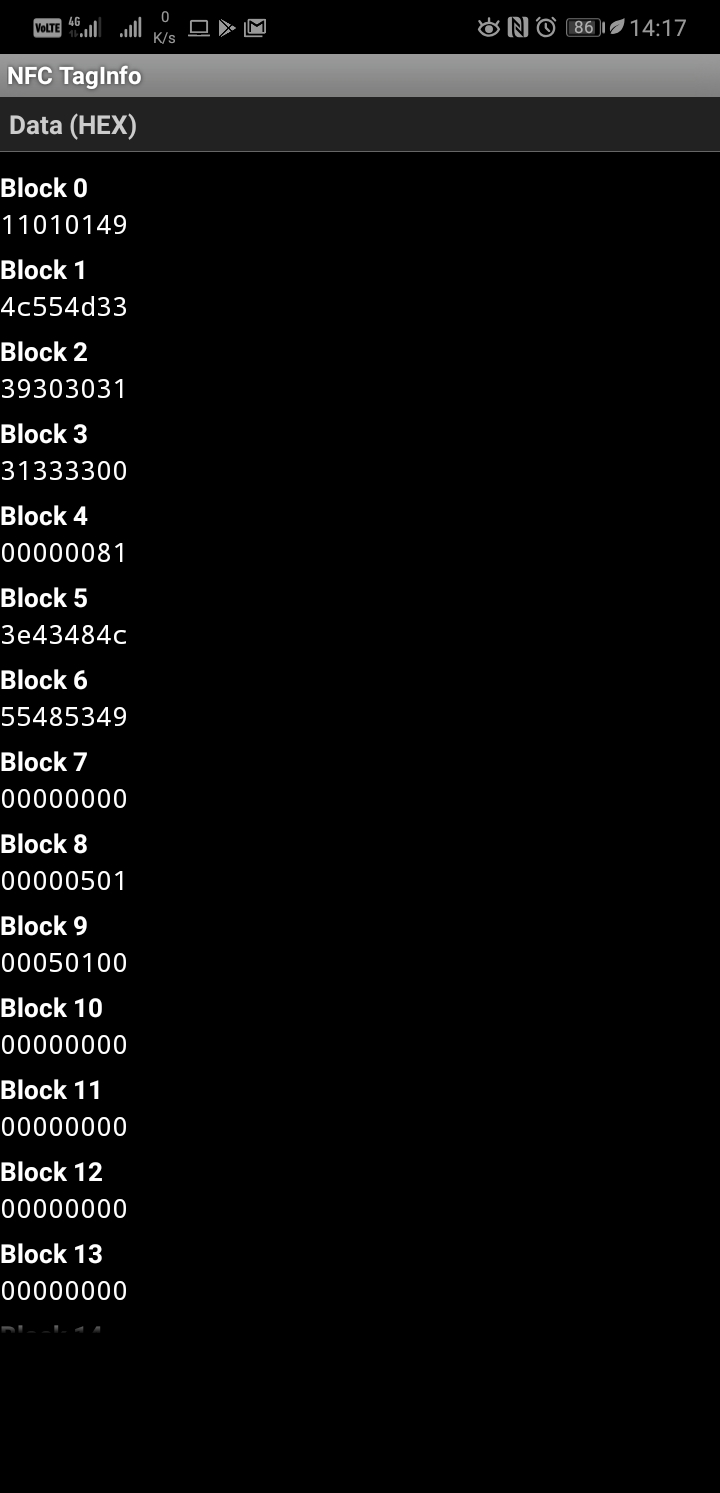
\includegraphics[keepaspectratio,width=\linewidth]{RFID_Blocks-Hex}
		\caption{Blöcke in Hex mit Smarphone ausgelesen}
	\end{subfigure}
	\begin{subfigure}[t]{.45\textwidth}
		\centering
		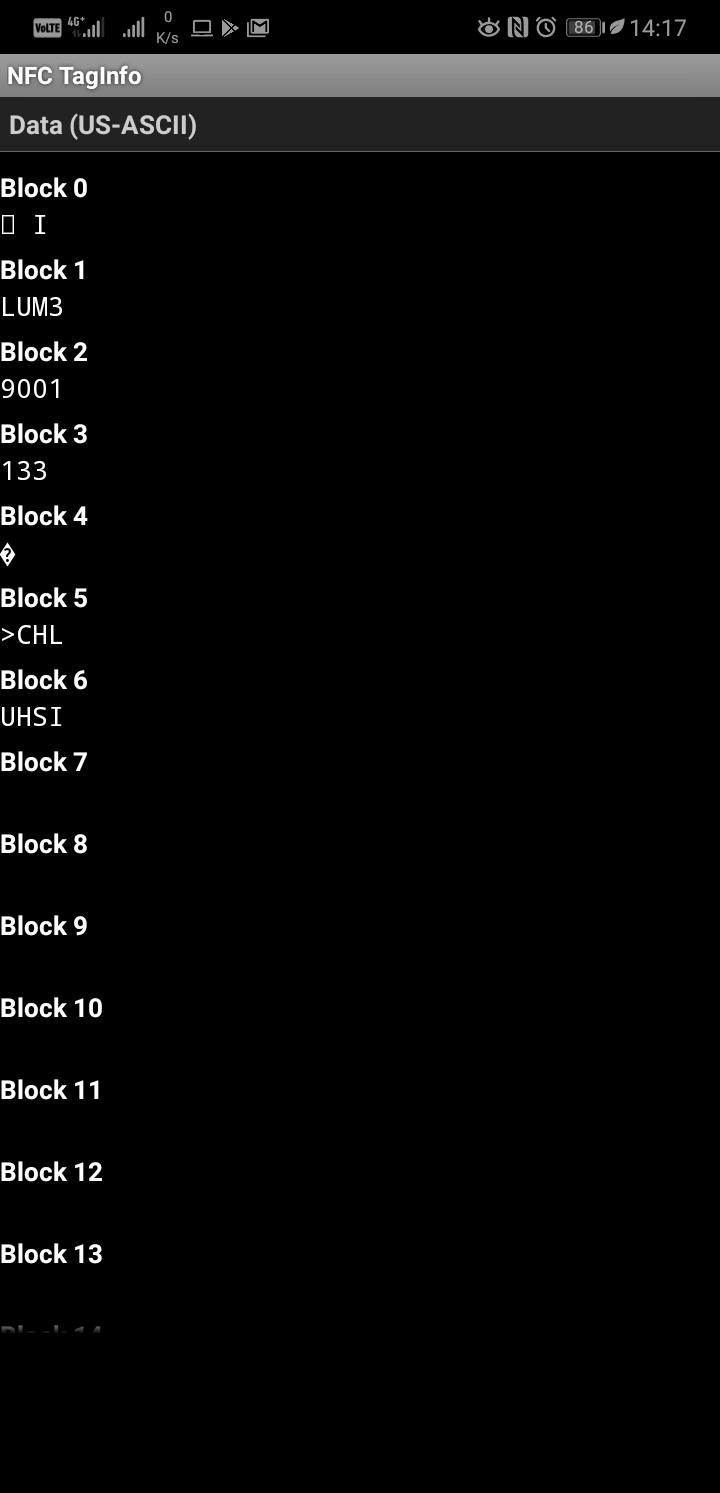
\includegraphics[keepaspectratio,width=\linewidth]{RFID_Blocks-Ascii}
		\caption{Blöcke in ASCII mit Smarphone ausgelesen}
	\end{subfigure}
	\begin{subfigure}[b]{.3\textwidth}
		\centering
		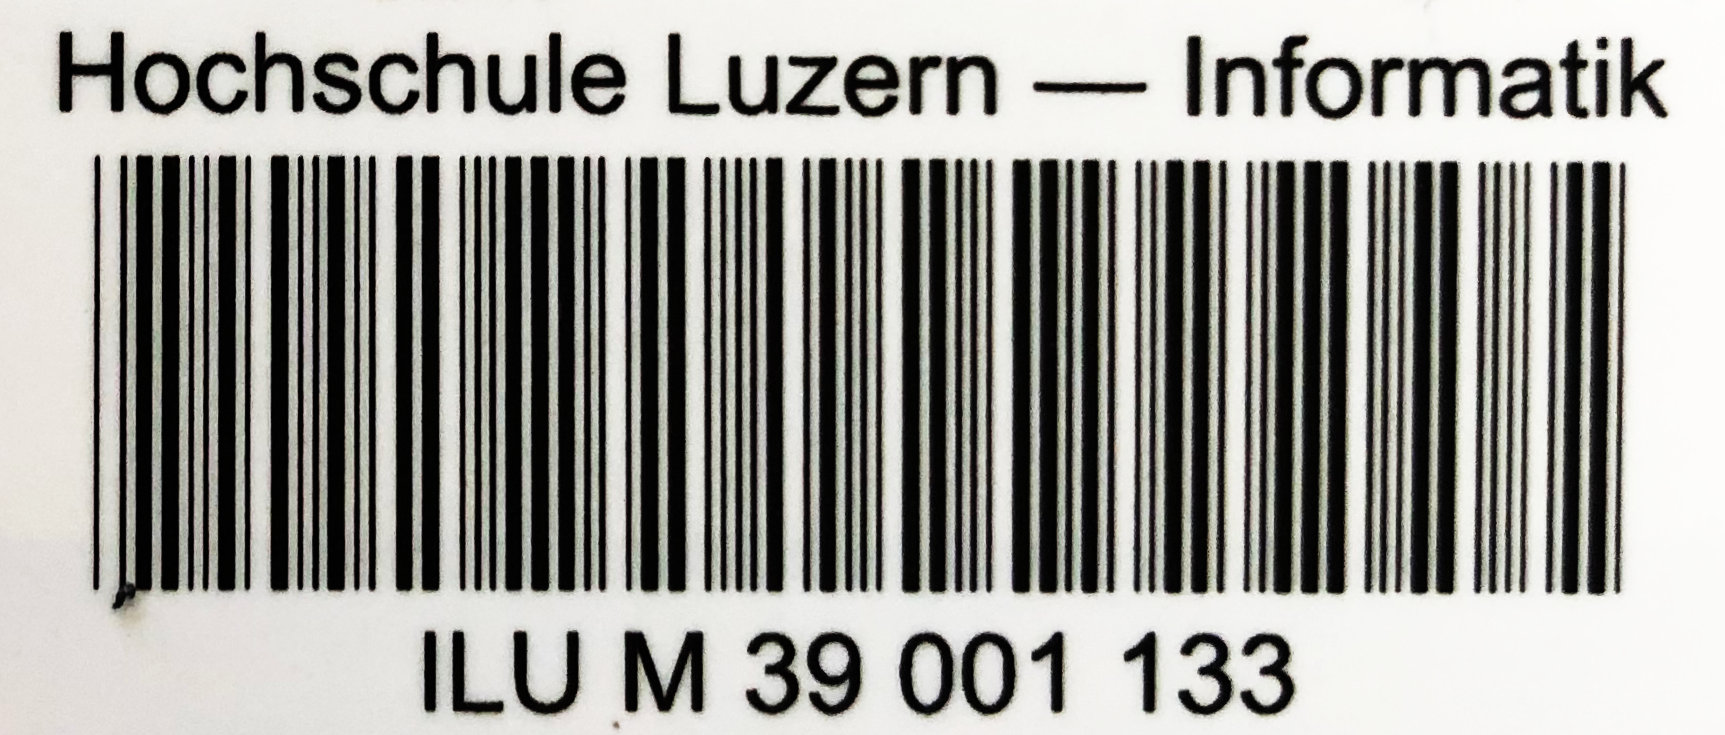
\includegraphics[keepaspectratio,width=\linewidth]{Barcode_BuchRFIDTag}
		\caption{Zugehöriger Barcode}
	\end{subfigure}
	\caption{Ausgelesene Blöcke und Barcode des Buches}
	\label{fig:AusgeleseneBloeckeUndBarcode}
\end{figure}


\clearpage
\section{Systemspezifikation Referenzimplementation}
\label{sec:SysSpec}

\subsection{Anforderungen}
\label{sub:ReferenzimplementationAnforderungen}
Hier werden die Anforderungen an die Referenzimplementation, welche bereits in Kapitel \ref{sub:Anforderungen} erwähnt wurden, nochmals aufgelistet.
\begin{legal}
	\item Die Referenzimplementation ist in der Lage die Buch ID eines Exemplares über RFID auszulesen.
	\item Die Referenzimplementation soll erkennen, wenn eine Box ein Exemplar (welches mit RFID ausgestattet ist und technisch auch Lesbar ist) enthält, welches nicht dieser Box zugehörig ist.
	\item Die Referenzimplementation soll jede erkannte Unstimmigkeit (Exemplar, welches nicht zu diesem Behälter gehört) in einem Logdokument persistieren.
	\item Die Referenzimplementation soll in der Lage sein, dem Endbenutzer, in graphischer Form durch eine Konsolen-Ausgabe, mitzuteilen, welcher Behälter eine Unstimmigkeit enthält.
	\item Die Referenzimplementation soll die unter Laborbedingungen erhaltenen Resultate unter Realbedingungen verifizieren.
	\item Die Referenzimplementation soll mit einer Oracle Datenbank kommunizieren können.
\end{legal}

\subsection{Kontext}

Das nachfolgende Kontextdiagramm (Abbildung \ref{fig:Kontextdiagramm}) beschreibt die Interaktion der Referenzimplementation mit allen Umsystemen. Diese Umsysteme bestehen aus dem Benutzer, welcher von der Referenzimplementation Informationen erhält, einem Datenbankexport Dokument, welches dem System die Informationen zu einem Exemplar liefert und dem RFID Reader, welcher der Referenzimplementation die Informationen eines gefundenen RFID Tags liefert.
\begin{figure}[htb]
	\centering
	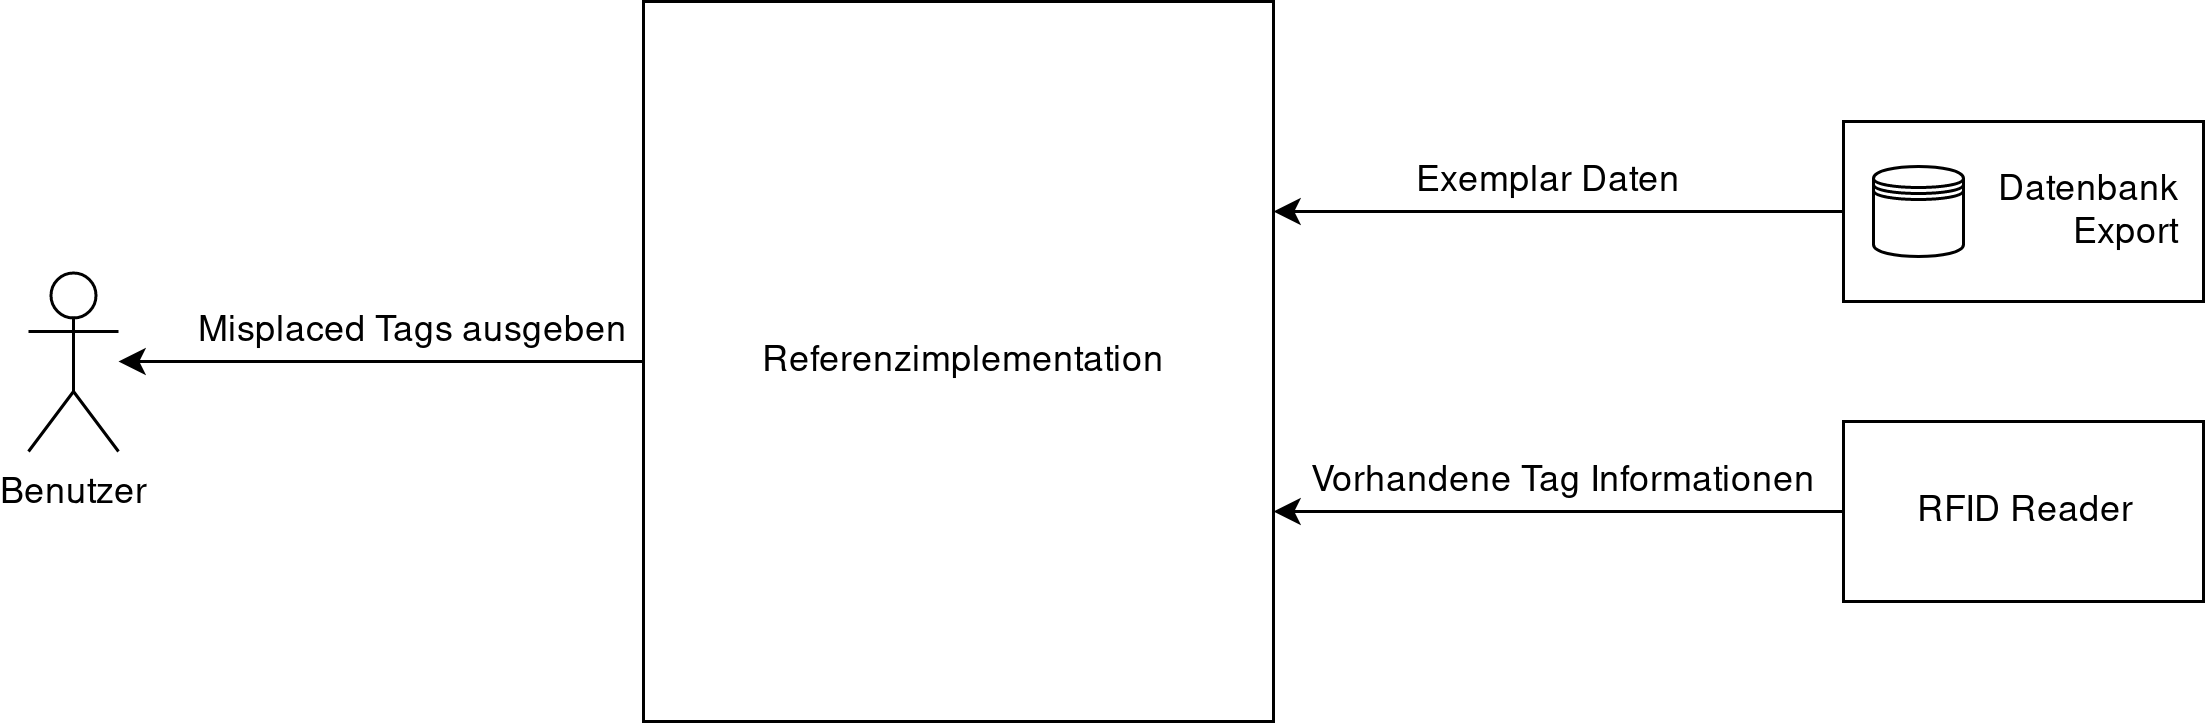
\includegraphics[keepaspectratio,width=.9\linewidth]{Kontextdiagramm}
	\caption{Kontextdiagramm der Referenzimplementation}
	\label{fig:Kontextdiagramm}
\end{figure}

\subsection{System}
Die folgende Darstellung \ref{fig:System} zeigt die Systeme auf, auf welcher die Referenzimplementation aufbaut.
Da die Referenzimplementation in Kotlin geschrieben wurde, wird eine Java Virtual Machine vorausgesetzt. Die notwendige Kommunikation zur RFID Hardware läuft über einen RFID Treiber, welcher nur als eine nicht verwaltete \gls{DLL} vom Hersteller zur Verfügung gestellt wird. Bei einer nicht verwalteten \gls{DLL} handelt es sich um eine Bibliothek, welche direkt zu Assembler Code kompiliert wird und daher nur auf der dafür kompilierten Architektur/Betriebssystemumgebung ausführbar ist. Diese, vom Hersteller gelieferte, nicht verwalteten \gls{DLL}, setzt voraus, dass sie auf einem Windows Betriebssystem im 32Bit Modus ausgeführt wird.
\begin{figure}[htb]
	\centering
	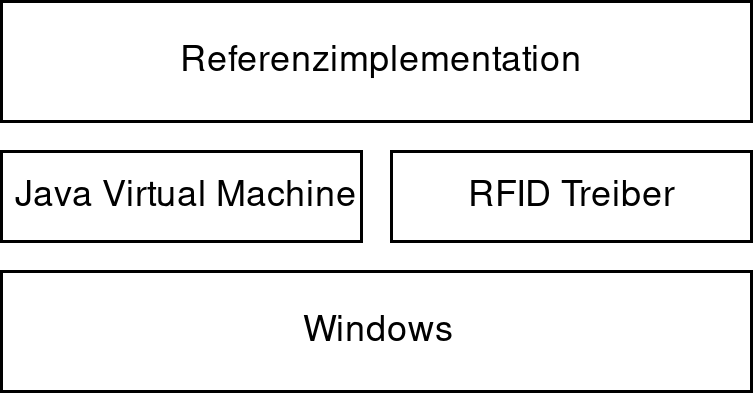
\includegraphics[keepaspectratio,width=.5\linewidth]{System}
	\caption{Darstellung der Systeme, von welcher die Referenzimplementation abhängt}
	\label{fig:System}
\end{figure}

\subsection{Komponenten}
Im folgenden Diagramm \ref{fig:Components} sind die entwickelten Softwarekomponenten abgebildet. Es zeigt in vereinfachter Form, dass zwischen den Hauptkomponenten UI, MisplacedTagIdentifier und TagReader keine starke Kopplung vorhanden ist.
\begin{figure}[htb]
	\centering
	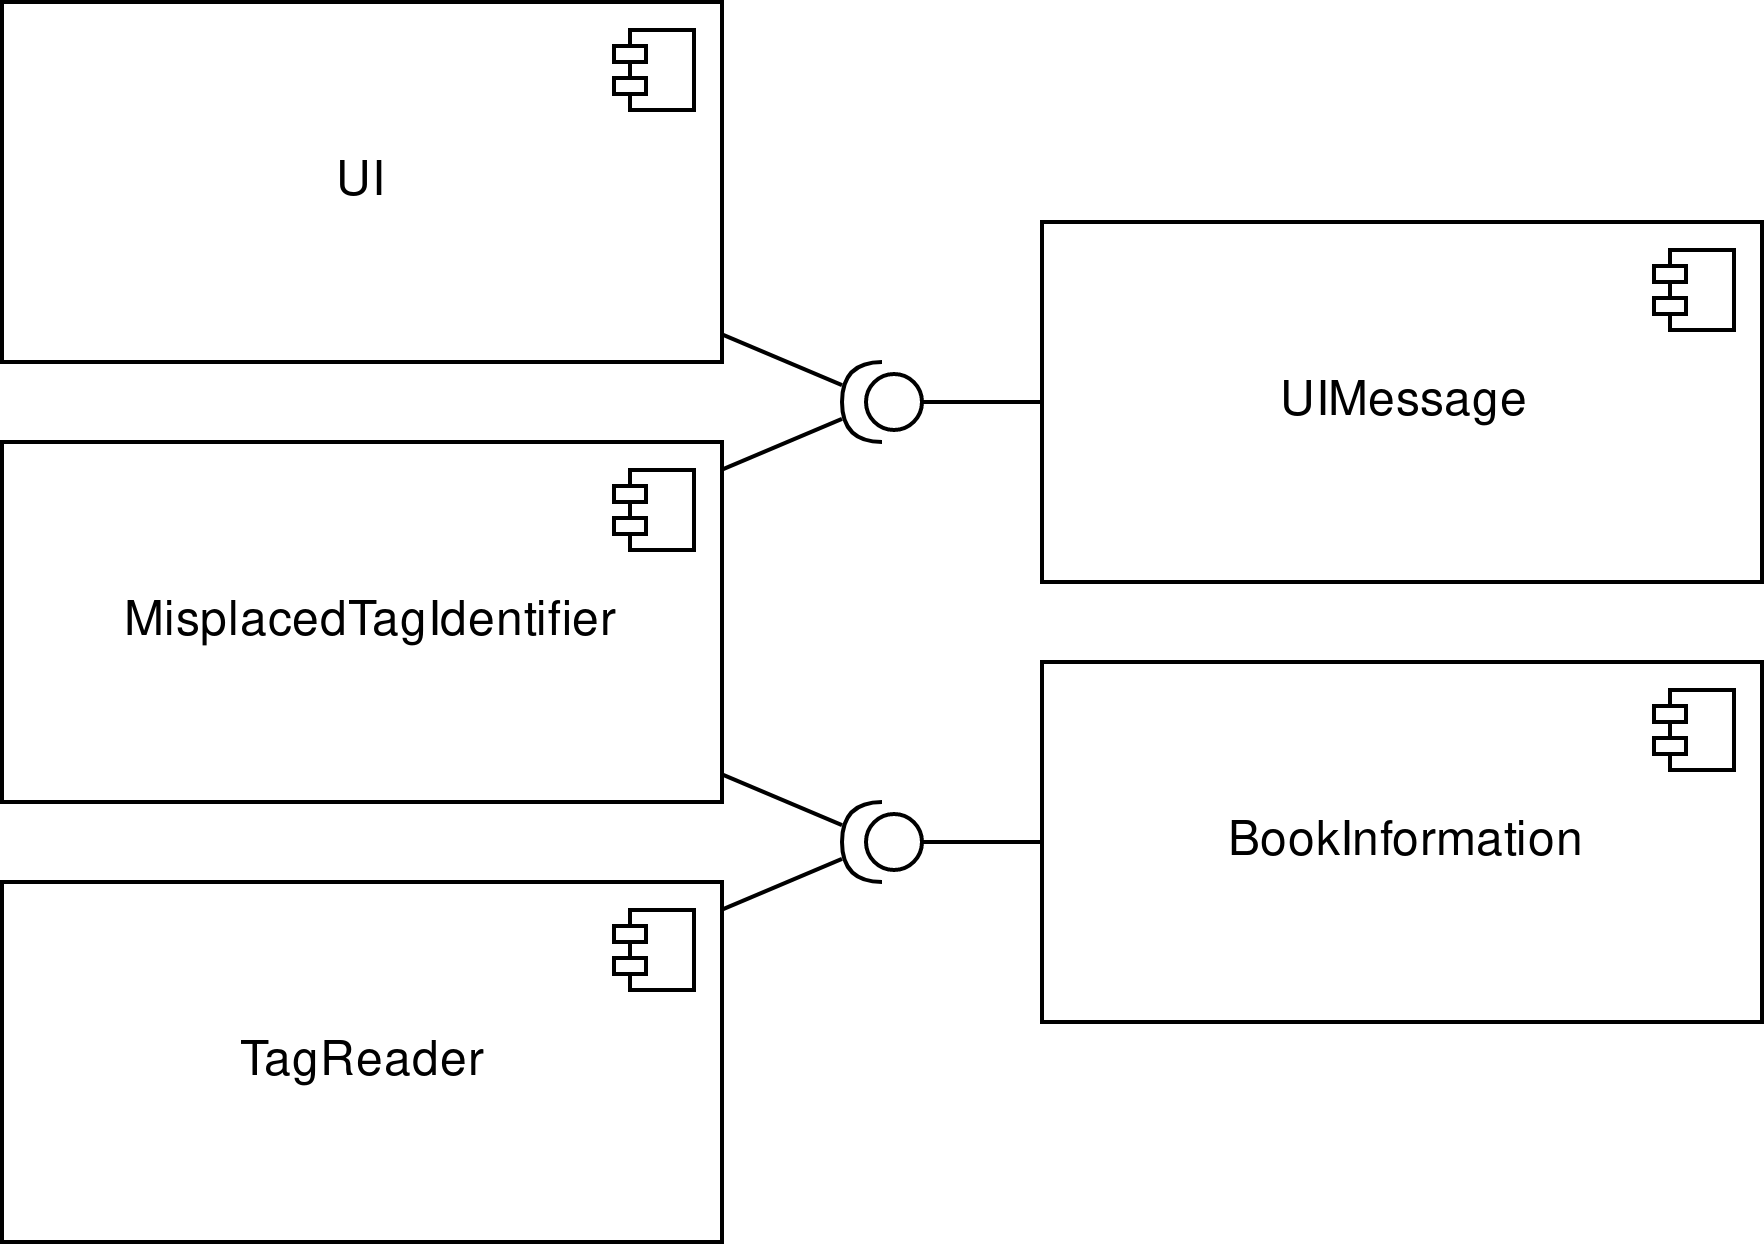
\includegraphics[keepaspectratio,width=.6\linewidth]{Komponentendiagramm}
	\caption{Darstellung der Klassen in der Komponente UI}
	\label{fig:Components}
\end{figure}

\clearpage
\subsubsection{UI}
In der Abbildung \ref{fig:ClassUI} ist das Klassendiagramm der Komponente UI zu sehen.
In diesem Diagramm ist ersichtlich, dass ein angepasstes MVC Pattern verwendet wird.
\begin{figure}[htb]
	\centering
	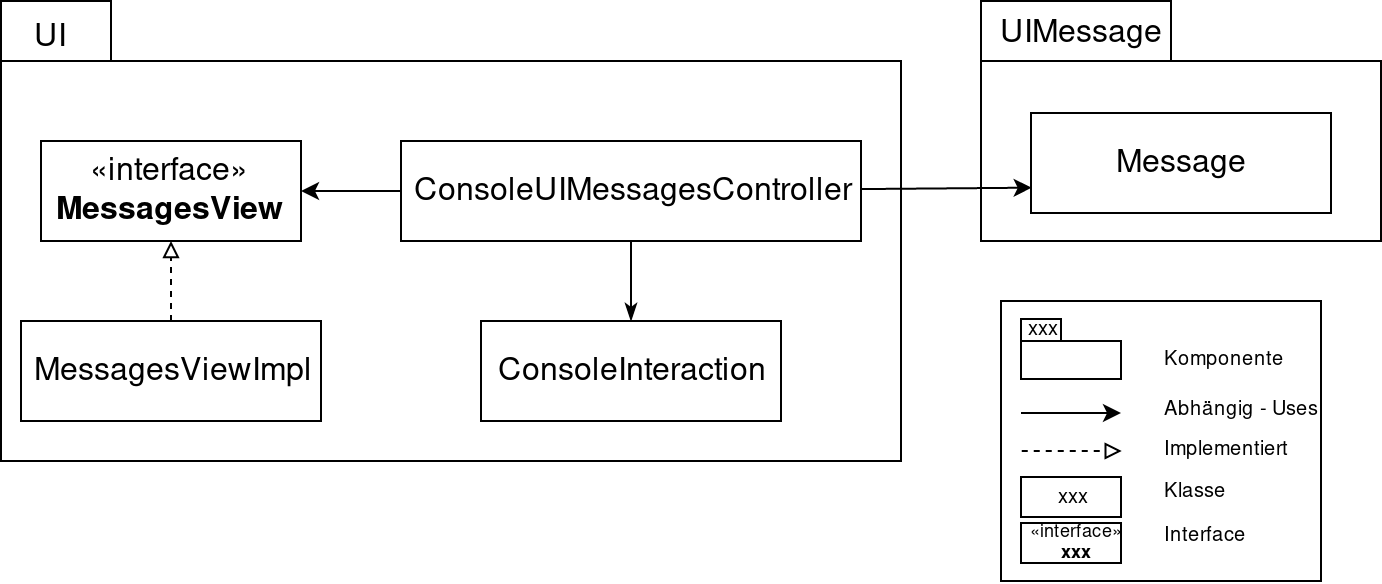
\includegraphics[keepaspectratio,width=\linewidth]{ClassdiagrammUI}
	\caption{Klassendiagramm der Komponente UI mit Darstellung der Abhängigkeit zu UI Message}
	\label{fig:ClassUI}
\end{figure}
\subsubsection{UI Message}
In der Abbildung \ref{fig:ClassUIMessage} ist das Klassendiagramm der Komponente UI Message zu sehen.
In diesem Diagramm ist ersichtlich, dass es nur eine Datenklasse in dieser Komponente gibt.
\begin{figure}[htb]
	\centering
	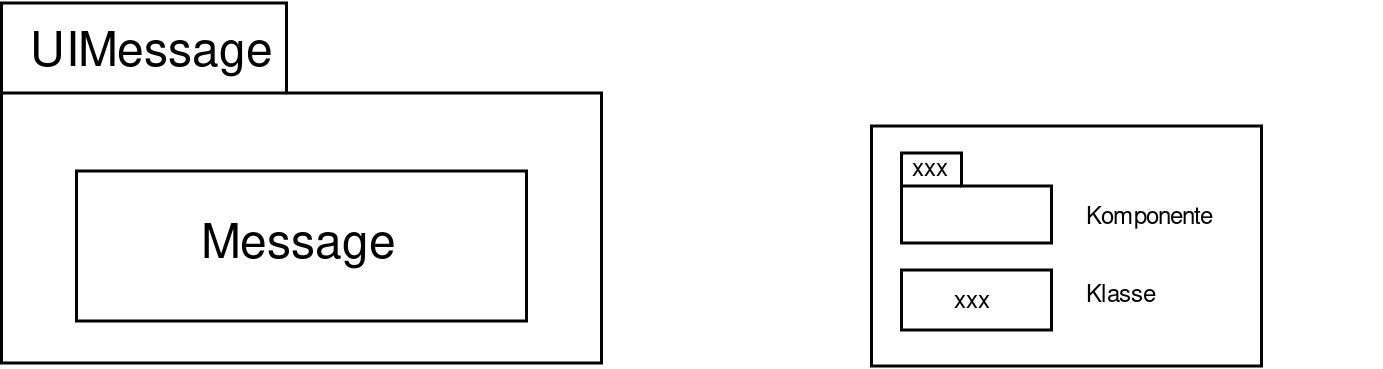
\includegraphics[keepaspectratio,width=.6\linewidth]{ClassdiagrammUIMessage}
	\caption{Klassendiagramm der Komponente UI Message}
	\label{fig:ClassUIMessage}
\end{figure}

\clearpage
\subsubsection{Misplaced Tag Identifier}
In der Abbildung \ref{fig:ClassMisplacedTagIdentifier} ist das Klassendiagramm der Komponente Misplaced Tag Identifier zu sehen.
In diesem Diagramm ist ersichtlich, dass der MisplacedTagIdentifyController die Rolle des Bindeglieds zwischen dem Logger (LogPersistor), dem Exemplar-Informationslieferanten (LibraryCopySupplier) und der Deplatzierungserkennung (MisplacedIdentifier) einnimmt.
\begin{figure}[htb]
	\centering
	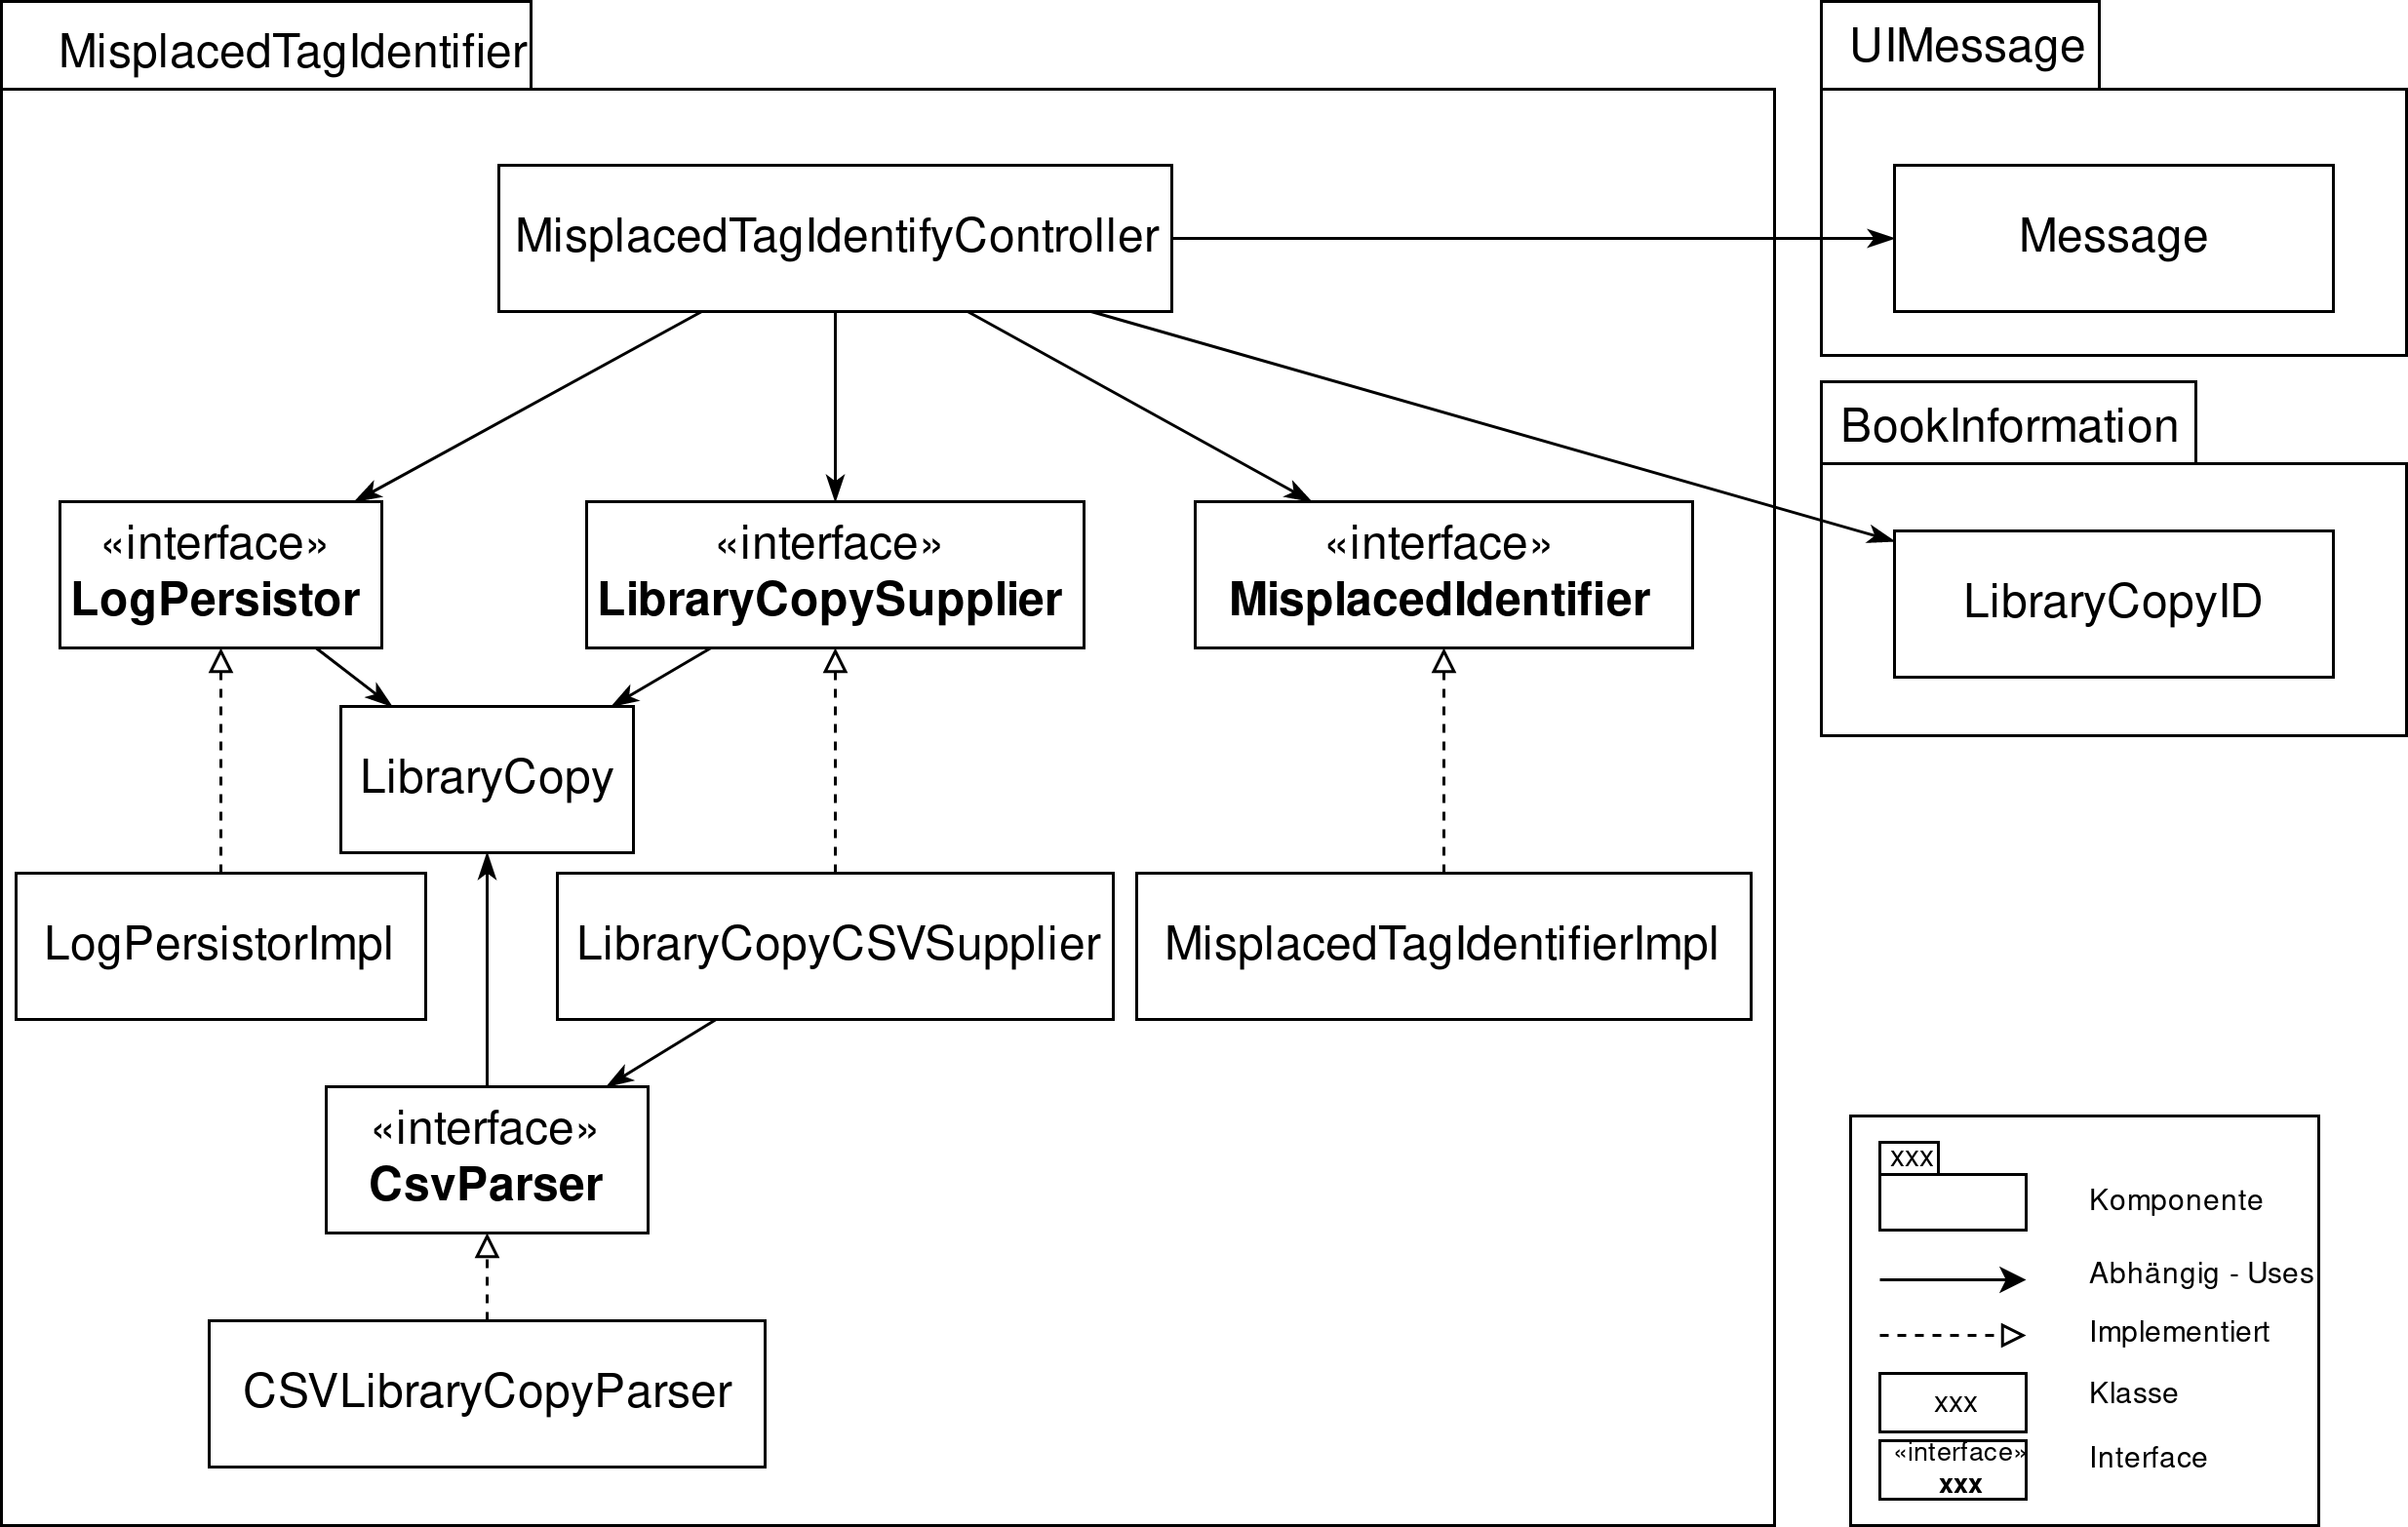
\includegraphics[keepaspectratio,width=\linewidth]{ClassdiagrammMisplacedTagIdentifier}
	\caption{Klassendiagramm der Komponente Misplaced Tag Identifier mit Darstellung der Abhängigkeit zu UI Message und Book Information}
	\label{fig:ClassMisplacedTagIdentifier}
\end{figure}

\subsubsection{Book Information}
In der Abbildung \ref{fig:ClassBookInformation} ist das Klassendiagramm der Komponente Book Information zu sehen.
In diesem Diagramm ist ersichtlich, dass es nur eine Datenklasse in dieser Komponente gibt.
\begin{figure}[htb]
	\centering
	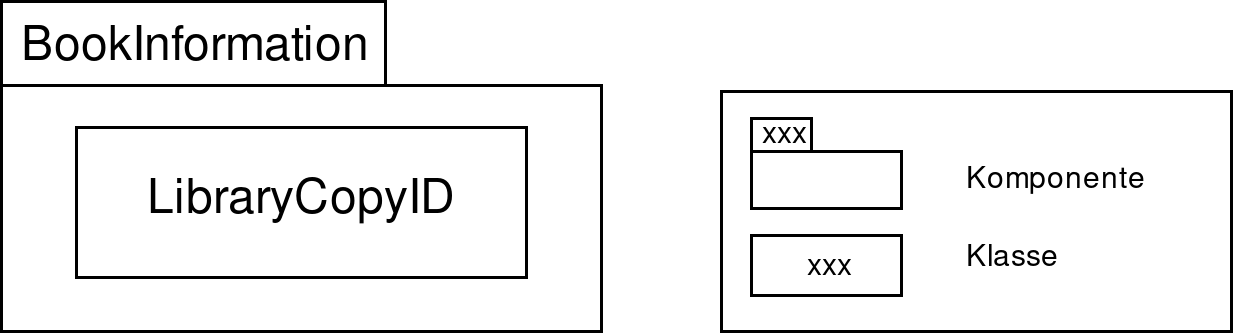
\includegraphics[keepaspectratio,width=.6\linewidth]{ClassdiagrammBookInformation}
	\caption{Klassendiagramm der Komponente Book Information}
	\label{fig:ClassBookInformation}
\end{figure}

\subsubsection{Tag Reader}
In der Abbildung \ref{fig:ClassTagReader} ist das Klassendiagramm der Komponente Tag Reader zu sehen.
In diesem Diagramm ist ersichtlich, dass für den CommunicationDriver das Adapter Pattern verwendet wurde. Dies ermöglichte, dass bereits vor der Hardwarelieferung mit der Implementation begonnen werden konnte. 

\begin{figure}[htb]
	\centering
	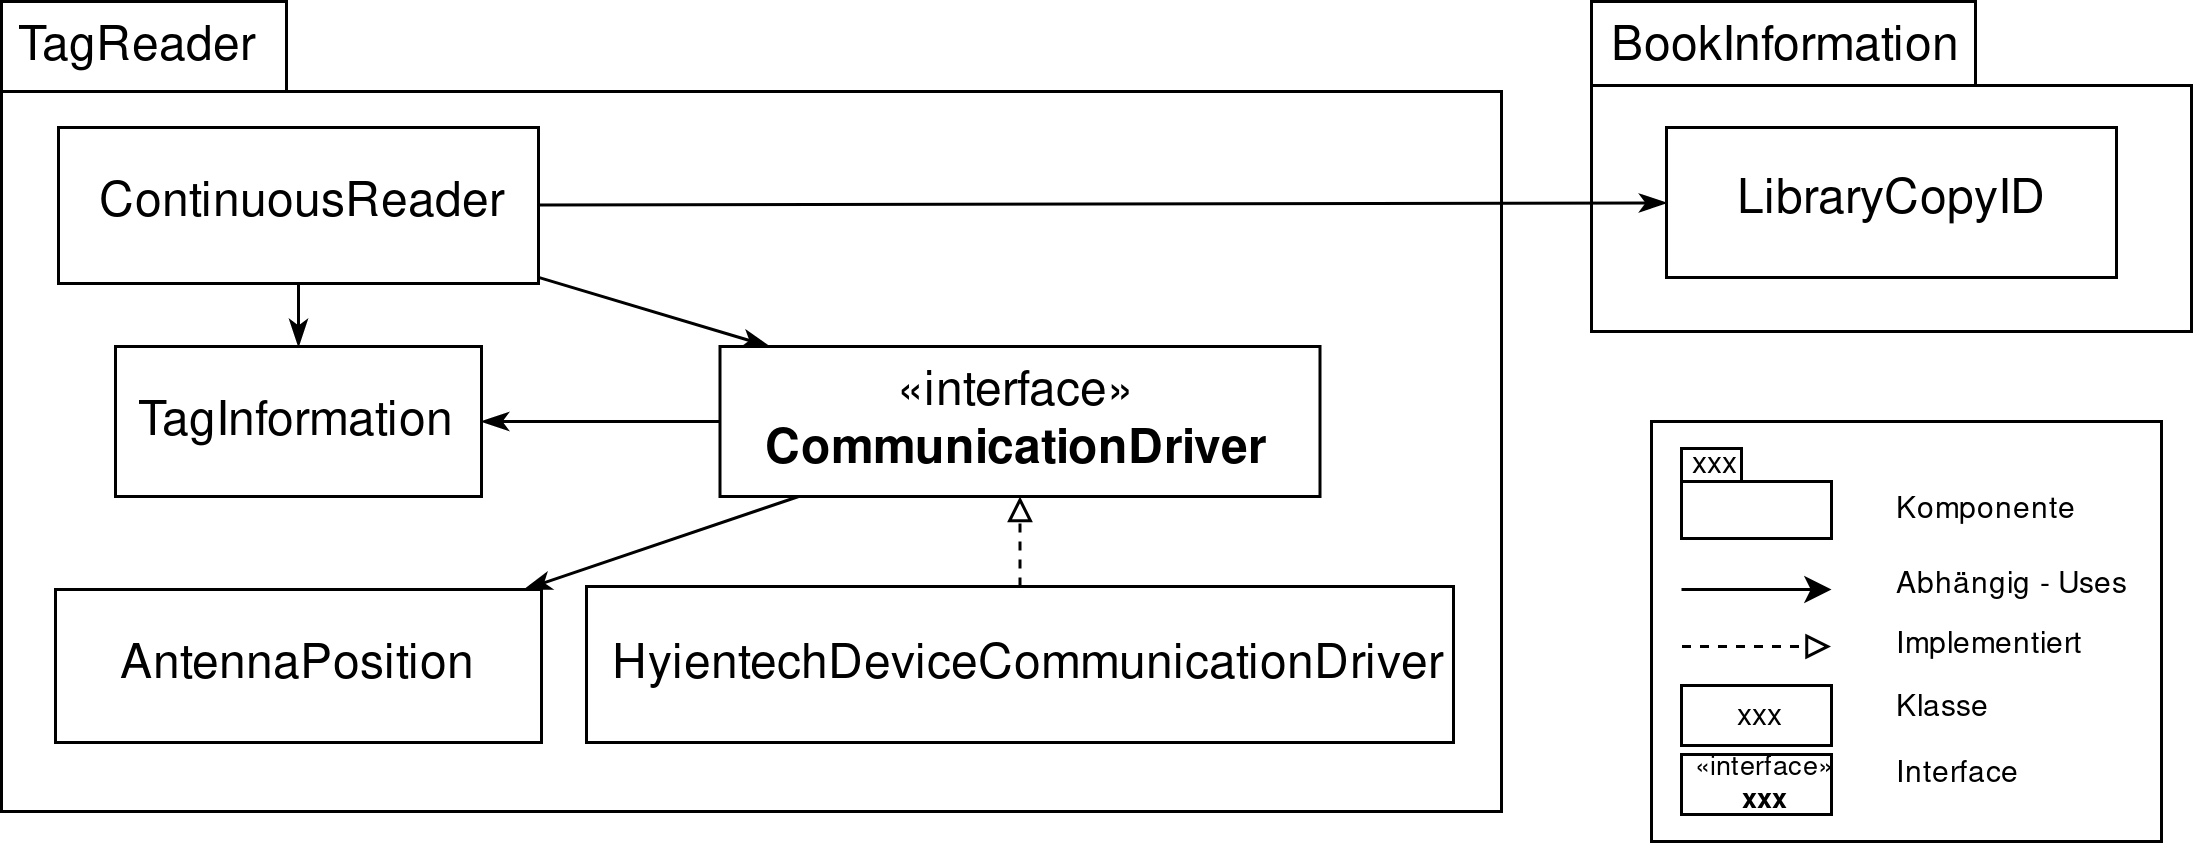
\includegraphics[keepaspectratio,width=\linewidth]{ClassdiagrammTagReader}
	\caption{Klassendiagramm der Komponente Tag Reader mit Darstellung der Abhängigkeit zu Book Information}
	\label{fig:ClassTagReader}
\end{figure}


\subsection{Ablauf Erkennung eines Tags}
Mit folgenden Diagramm \ref{fig:AblaufdiagrammTagErkennung} wird der Ablauf dargelegt, welcher die Referenzimplementation durchläuft, sobald ein Tag Identifiziert werden konnte. Der Wechsel von einer Komponenten zur nächsten wird durch ein Benachrichtigungssystem ermöglicht. Als Benachrichtigungssystem wurde die ConcurrentLinkedQueue, welche mit der Standard Bibliothek von Kotlin zur Verfügung gestellt wird, eingesetzt. 
\begin{figure}[htb]
	\centering
	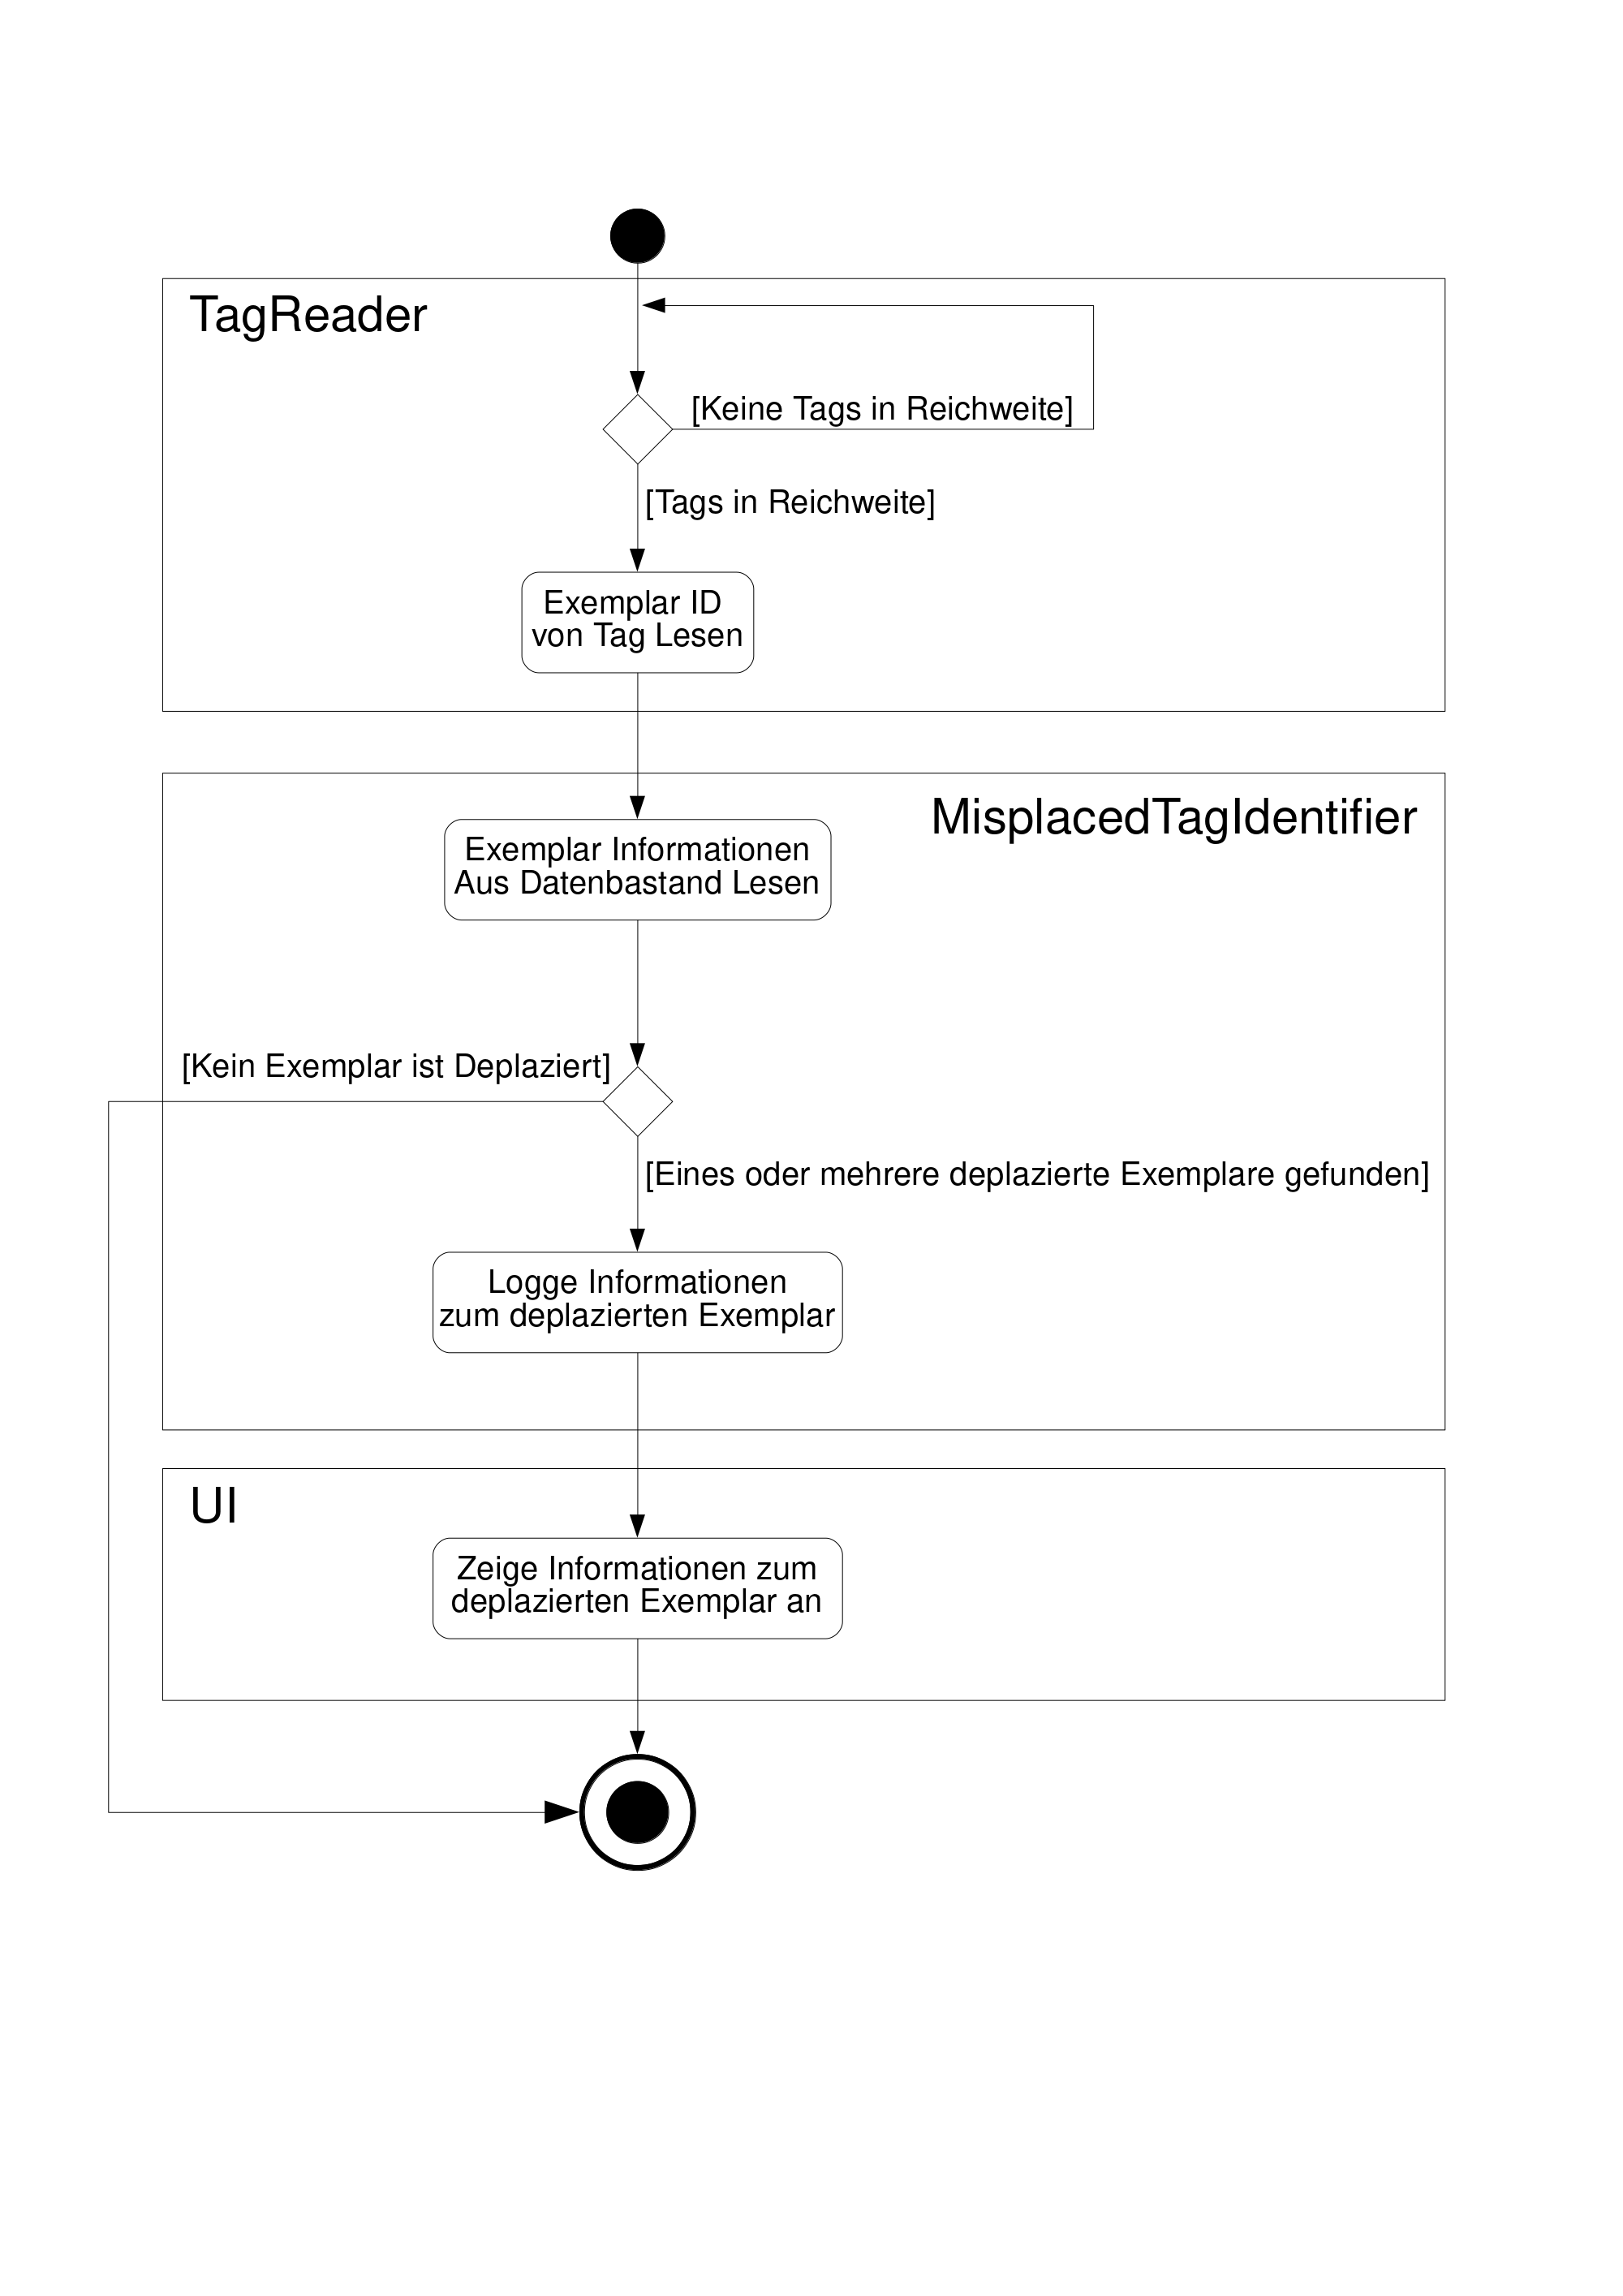
\includegraphics[keepaspectratio,width=.8\linewidth]{AblaufdiagrammTagErkennung}
	\caption{Ablaufdiagramm zur Tag-Erkennung mit Darstellung, welcher Ablauf in welcher Komponenten erfolgt}
	\label{fig:AblaufdiagrammTagErkennung}
\end{figure}

\clearpage
\subsection{Umsetzung Programmierung}
\subsubsection{Clean Code}
Gut lesbarer Code ist verständlicher als veraltete, nicht akkurate Kommentare. Diesem Zustand haben wir entgegengesetzt, indem wir auf JavaDoc, sowie nicht notwendige Kommentare verzichtet haben. Dieser Entscheid hatte zur Folge, dass eine sprechende Namensgebung für alle zu benennende Elemente im Code verwendet wurden. Weiter wurden starke Verschachtelungsebene in einzelne Funktionen unterteilt, sowie Klassen eher klein gehalten (\cite{martin2009clean}).

\subsubsection{Feature Branch Workflow}
Um möglichst effizient und unabhängig voneinander zu programmieren, sowie zu dokumentieren, wurde mit dem Feature Branch Workflow gearbeitet. Dies bedeutet, dass für jedes Feature einen Branch erstellt wurde. Weiter wurde eine Regelung eingeführt, wobei ein Branch nicht vom Ersteller mit dem Master Branch zusammengeführt werden darf. Um diese Regel zu erzwingen, wurde der Master Branch auf GitHub für alle Projekte entsprechend geschützt. Durch diesen Schritt, konnten wir die Sicherheit erhöhen, da eine zweite Person ein Review der Dokumentation, respektive des Codes durchführen muss.
Auf der Abbildung \ref{fig:FeatureBranchWorkflow} ist ein Auszug aus der Baumstruktur unserer Dokumentation dargestellt. Dabei ist zu erkennen, dass zu Sprintbeginn möglichst keine offenen Zweige (engl. Branches) mehr vorhanden sind und gegen Sprintende alle Zweige in den Master (in Abbildung \ref{fig:FeatureBranchWorkflow} schwarz dargestellt) über einen Pull Request zusammengeführt werden(\cite{BaumannWicki2018}).

\begin{figure}[htb]
	\center
	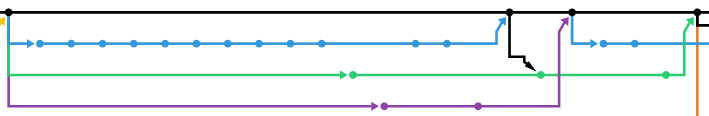
\includegraphics[width=\textwidth]{GitFeatureBranchWorkflow}
	\caption{Branches unsere Dokumentation aus Sprint 5}
	\label{fig:FeatureBranchWorkflow}
\end{figure}
